\documentclass[crop, tikz]{standalone}

\usepackage[utf8]{inputenc}
% 'crop' is the default for v1.0, before it was 'preview'
%\usetikzlibrary{...}% tikz package already loaded by 'tikz' option

\usetikzlibrary{arrows}
\usetikzlibrary{decorations.markings}
\usetikzlibrary{patterns}
\usetikzlibrary{calc}

\begin{document}
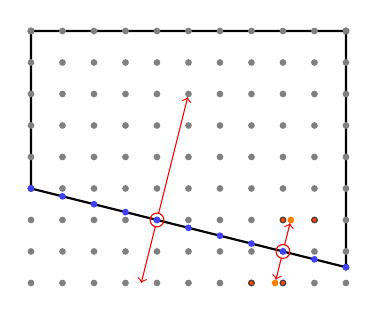
\begin{tikzpicture}
	% draw nodes
	\filldraw[black] (0,0) circle [radius=1pt];
	\filldraw[black] (0,2) circle [radius=1pt];
	\filldraw[black] (4,2) circle [radius=1pt];
	\filldraw[black] (4,-1) circle [radius=1pt];
	
	% draw region outline
	\draw[thick, black] (0,0) -- (0,2) -- (4,2) -- (4,-1) -- cycle;

	% draw new mesh, where we have placed extra nodes along the skeleton and at the vertex
	\foreach \x in {0,0.4,...,4} {
		\foreach \y in {0,0.4,...,2} {
			\filldraw[black!50!white] (\x,\y) circle [radius=1pt];
		}
		\foreach \y in {-0.4,-0.8,...,-1.3} {
			\filldraw[black!50!white] (\x,\y) circle [radius=1pt];	
		}
	}
	\foreach \x in {0,0.4,...,4} {
		\filldraw[blue!75!white] (\x,-0.25*\x) circle [radius=1pt];
	}

	% the closest "adjacent" node might be quite far away!
	\draw[red] (1.6,-0.4) circle [radius=2.5pt];
	\draw[red, ->] (1.6+0.02,-0.4+4*0.02) -- (2-0.01,1.2-4*0.01);
	\draw[red, ->] (1.6-0.02,-0.4-4*0.02) -- (1.4,-1.2);
	% maybe approximating via interpolation is better?
	\draw[red] (3.2,-0.8) circle [radius=2.5pt];
	% interpolated nodes
	\filldraw[red!50!yellow] (3.3,-0.4) circle [radius=1pt];
	\filldraw[red!50!yellow] (3.1,-1.2) circle [radius=1pt];
	\draw[red, ->] (3.2+0.02,-0.8+4*0.02) -- (3.3-0.01,-0.4-4*0.01);
	\draw[red, ->] (3.2-0.02,-0.8-4*0.02) -- (3.1+0.01,-1.2+4*0.01);
	% highlight nodes contributing to the interpolation
	\filldraw[fill=red!75!yellow, draw=black!75!white] (3.2,-0.4) circle [radius=1pt];
	\filldraw[fill=red!75!yellow, draw=black!75!white] (3.6,-0.4) circle [radius=1pt];
	\filldraw[fill=red!75!yellow, draw=black!75!white] (2.8,-1.2) circle [radius=1pt];
	\filldraw[fill=red!75!yellow, draw=black!75!white] (3.2,-1.2) circle [radius=1pt];
\end{tikzpicture}
\end{document}